\documentclass[12pt,a4paper,oneside]{report}

% =========================
% Packages
% =========================

\usepackage[utf8]{inputenc}
\usepackage[T1]{fontenc}
\usepackage[french]{babel}

\usepackage{graphicx}
\usepackage{float}
\usepackage{array}
\usepackage{longtable}
\usepackage{booktabs}
\usepackage{tabularx}
\usepackage{colortbl}
\usepackage{caption}
\usepackage{subcaption}

\usepackage{amsmath}
\usepackage{amssymb}

\usepackage{pdfpages}
\usepackage{pdflscape}
\usepackage{hyperref}
\usepackage{xcolor}
\usepackage{geometry}

\definecolor{headblue}{HTML}{2E75B6}
\definecolor{rowgray}{HTML}{EBF3FA}

\geometry{
    a4paper,
    left=2cm,
    right=2cm,
    top=1.8cm,
    bottom=3cm
}

\usepackage{setspace}
\onehalfspacing

\usepackage{titlesec}
\usepackage{fancyhdr}
\usepackage{minitoc}
\usepackage{calc}

% =========================
% BIBLIOGRAPHIE
% =========================

\usepackage[backend=biber,style=ieee]{biblatex}

\addbibresource{bibliographie/biblio.bib}
\addbibresource{bibliographie/references.bib}

% NE PAS mettre \nocite{*} ici — on le met juste avant chaque \printbibliography

% =========================
% Header & Footer
% =========================

\pagestyle{fancy}
\fancyhf{}
\fancyhead[L]{\nouppercase{\leftmark}}
\fancyfoot[C]{\thepage}

\renewcommand{\headrulewidth}{0.4pt}
\renewcommand{\footrulewidth}{0.4pt}

% =========================
% TOC
% =========================

\setcounter{tocdepth}{3}
\setcounter{secnumdepth}{3}

% =========================
% MINITOC
% =========================

\dominitoc

% =========================
% STYLE CHAPITRE (INTACT)
% =========================

\makeatletter

\newlength{\chapter@number@width}

\def\@makechapterhead#1{%
  {%
  \normalfont
  \setlength{\parindent}{0pt}%
  \vspace*{10pt}%

  \settowidth{\chapter@number@width}{%
    \hbox{%
      \color{white}\Large\bfseries
      \hspace{\dimexpr 1mm+3pt}%
      \thechapter
      \hspace{\dimexpr 1mm+3pt}%
    }%
  }

  \hbox{

    % Bloc gauche
    \vtop{%
      \hsize=\dimexpr\chapter@number@width+\tabcolsep+2\fboxrule+\tabcolsep

      \begin{tabular}[t]{@{}c}
        \scshape
        \@chapapp

        \fboxsep=0pt
        \colorbox{black}{%
          \vbox{
            \hbox{\vbox to 0.7cm{}}
            \hbox{%
              \color{white}\Large\bfseries
              \thechapter
            }
            \hbox{\vbox to 5pt{}}
          }%
        }

      \end{tabular}%
    }%

    % Bloc droite
    \vtop{%
      \advance\hsize by -\dimexpr\chapter@number@width
      \hspace*{-0.4cm}

      \begin{tabular}[t]{c}
        \scshape

        \fboxsep=0pt
        \colorbox{white}{%
          \vbox{

            \hbox{\Large\bfseries #1}

          }%
        }

      \end{tabular}%
    }%
  }%

  \vspace{40pt}
  }%
}

\makeatother

% =========================
% DOCUMENT
% =========================

\begin{document}

% --- Page de garde (pas de numéro) ---

\includepdf[pages=-]{page_garde.pdf}

% --- Pages préliminaires en chiffres romains ---
\pagenumbering{roman}
\pagestyle{fancy}

\clearpage
\chapter*{Remerciements}
\markboth{Remerciements}{Remerciements}

\begin{center}
\begin{minipage}{0.9\textwidth}
\centering
\small
\setstretch{1.12}

Au terme de ce travail, je tiens à exprimer ma profonde gratitude à toutes les personnes qui ont contribué, par leur accompagnement, leurs conseils et leur soutien, à la réalisation de ce projet de fin d'études.

Je tiens à adresser mes sincères remerciements à mon encadrante académique, Mme \textbf{Sihem LOUKIL}, pour son accompagnement, ses conseils avisés et l'intérêt qu'elle a porté à l'évolution de ce travail. Ses remarques m'ont aidée à prendre du recul sur mes choix, à organiser mes idées avec plus de rigueur et à améliorer la présentation de ce projet.

J'adresse également mes sincères remerciements à mon encadrant industriel, M. \textbf{Hazem RAOUAFI}, pour son suivi, sa confiance et les orientations qu'il m'a apportées tout au long de mon stage. Son accompagnement m'a permis de mieux comprendre les besoins du projet et d'avancer de manière plus structurée dans la réalisation de la plateforme.

Je remercie également l'ensemble de l'équipe de la société \textbf{3S} qui nous a accompagnés durant cette expérience. Leur accueil, leur disponibilité et leurs échanges m'ont permis d'évoluer dans un cadre professionnel enrichissant et de mieux comprendre les attentes concrètes liées au projet.

Je tiens à exprimer ma reconnaissance à la société \textbf{Standard Sharing Software (3S)} pour m'avoir offert l'opportunité d'effectuer mon stage de fin d'études dans un environnement professionnel, stimulant et enrichissant. Cette expérience m'a permis de mettre en pratique mes connaissances, de développer de nouvelles compétences et de travailler sur un sujet concret répondant à des besoins réels.

Enfin, j'adresse mes respectueux remerciements aux membres du jury pour l'honneur qu'ils me font en acceptant d'évaluer ce travail et pour l'attention qu'ils porteront à ce mémoire.

\end{minipage}
\end{center}


\clearpage
\tableofcontents

\clearpage
\listoffigures

\clearpage
\listoftables

% --- Corps du document en chiffres arabes ---
\clearpage
\pagenumbering{arabic}
\setcounter{page}{1}

\clearpage
\chapter*{Introduction générale}
\markboth{Introduction générale}{Introduction générale}
\addtocontents{toc}{\protect\contentsline{introduction}{Introduction générale}{\thepage}{intro.1}}

Dans un contexte professionnel en constante mutation, où la transformation numérique et l'intelligence artificielle redéfinissent les modes d'apprentissage et de gestion des compétences, la formation continue devient un levier stratégique essentiel pour les entreprises. L'émergence de l'intelligence artificielle générative et des systèmes multi-agents ouvre aujourd'hui de nouvelles perspectives pour concevoir des plateformes d'apprentissage plus intelligentes, adaptatives et personnalisées.

C'est dans cette dynamique que s'inscrit notre projet de fin d'études, réalisé au sein de la société Standard Sharing Software (3S), acteur majeur de l'intégration de solutions technologiques en Tunisie et en Afrique. Ce projet vise à concevoir et développer une plateforme web intelligente de formation et de mentorat, capable de centraliser la gestion des compétences des collaborateurs du Groupe 3S tout en offrant un accompagnement pédagogique personnalisé basé sur l'intelligence artificielle.

La solution proposée repose sur une architecture microservices multi-tenant intégrant plusieurs agents intelligents spécialisés, chacun ayant un rôle précis dans le processus d'apprentissage : génération de contenus pédagogiques, coaching personnalisé, recommandation de ressources, suivi des apprenants et gestion de la mémoire contextuelle. Ces agents s'appuient sur des modèles de langage avancés, un système de Retrieval-Augmented Generation (RAG) agentique, ainsi qu'un mécanisme de mémoire persistante permettant d'assurer un suivi cohérent et évolutif des utilisateurs.

Ce rapport présente l'ensemble des travaux réalisés au cours de ce projet et s'articule autour de cinq chapitres principaux, chacun mettant en évidence une étape clé de la démarche.

Le premier chapitre, intitulé « Contexte général et méthodologie de travail », présente le cadre du projet, l'organisme d'accueil ainsi que la problématique étudiée. Il expose également les exigences fonctionnelles et non fonctionnelles, ainsi que la méthodologie de développement adoptée.

Le deuxième chapitre, « Concepts de base et étude préalable », introduit les fondements théoriques liés à l'intelligence artificielle générative, aux grands modèles de langage, aux systèmes multi-agents et aux approches de type RAG, qui constituent la base scientifique du projet.

Le troisième chapitre, « Conception et architecture de la plateforme », décrit l'architecture globale du système, notamment l'organisation en microservices, le modèle multi-tenant, ainsi que la conception des agents intelligents et les choix technologiques retenus.

Le quatrième chapitre, « Réalisation », présente les différents modules développés ainsi que les fonctionnalités implémentées, en mettant l'accent sur les composants liés à l'intelligence artificielle, à la gestion des formations et à l'expérience utilisateur.

Le cinquième chapitre, « Tests et validation », détaille la stratégie de test adoptée ainsi que les résultats obtenus à travers les tests unitaires, fonctionnels et de performance, ainsi que l'évaluation des modules d'intelligence artificielle.

Enfin, la conclusion générale synthétisera les apports du projet, évaluera le niveau d'atteinte des objectifs fixés et proposera des perspectives d'amélioration et d'évolution future de la plateforme.

\chapter{Contexte général et étude de l’existant}

\minitoc

\newpage

\section{Introduction}

Ce chapitre a pour objectif de présenter le cadre général du projet de fin d’études. 
Nous commençons par une présentation de l’entreprise d’accueil ainsi que de ses principaux domaines d’activité. 
Ensuite, nous étudions les solutions existantes dans le domaine concerné afin d’identifier leurs limites et les améliorations possibles. 
Enfin, nous présentons les exigences du projet ainsi que la méthodologie de travail adoptée durant sa réalisation.

% =====================================================




\section{Présentation de la société}

Cette section est consacrée à la présentation de la société d'accueil au sein de laquelle ce projet a été réalisé. Nous y décrivons son historique, son positionnement dans l'écosystème technologique tunisien ainsi que ses principaux domaines d'intervention.

% =====================================================

\subsection{Présentation générale}

Standard Sharing Software, désignée sous l'acronyme \textbf{3S} \cite{site3s}, est une entreprise tunisienne fondée en 1988, spécialisée dans l'intégration de solutions technologiques et les services informatiques à forte valeur ajoutée. Forte de plus de 35 ans d'expérience, elle s'est imposée comme un acteur de référence sur le marché tunisien et africain, en accompagnant les organisations publiques et privées dans leurs projets de modernisation numérique.

3S se distingue par une approche globale qui couvre l'ensemble du cycle de vie des projets IT : de l'étude et de l'audit des besoins jusqu'au déploiement et au pilotage des solutions mises en place. Cette capacité à intervenir de bout en bout, combinée à des partenariats avec des éditeurs et constructeurs de renommée mondiale, lui permet de proposer des réponses adaptées aux exigences les plus complexes.

\subsection{Positionnement au sein du Groupe 3S}

3S est la filiale fondatrice du \textbf{Groupe 3S} \cite{site3sgroup}, un groupe technologique tunisien structuré autour de deux pôles complémentaires. Le \textbf{pôle IT} regroupe les filiales dédiées aux technologies de l'information : \textbf{3S} (intégration IT), \textbf{GlobalNet} (accès Internet grand public), \textbf{GlobalNet Business} (services cloud et sécurité pour entreprises), \textbf{Advancia Training} (formation et certification IT), \textbf{Smartup} (édition de progiciels), \textbf{Hexabyte} (connectivité et solutions high-tech), \textbf{Cyberesa} (solutions e-tourisme) et \textbf{Pro2C} (centre de contact multicanal). Le \textbf{pôle Cleantech} quant à lui rassemble des entités orientées développement durable, telles que \textbf{Africa Solar} (énergies renouvelables), \textbf{CandyLed} (éclairage LED), \textbf{BioPack} (bioplastiques) et \textbf{Océane} (construction navale).

% =====================================================



\subsection{Domaines d'activité de 3S}

En tant que pôle IT du groupe, 3S intervient sur l'ensemble de la chaîne de valeur liée à la transformation numérique des entreprises. Ses domaines d'activité s'articulent autour de six axes principaux :

\begin{itemize}

    \item \textbf{Intégration des infrastructures IT :}
    3S accompagne ses clients dans la conception et le déploiement d'environnements informatiques robustes et évolutifs, conformes aux standards internationaux, depuis l'audit initial jusqu'à la mise en production ;

    \item \textbf{Réseaux et connectivité :}
    l'entreprise propose des solutions d'interconnexion et de télécommunication garantissant des échanges fiables et sécurisés entre les différents composants des systèmes d'information ;

    \item \textbf{Datacenter et continuité de service :}
    virtualisation, sauvegarde, stockage et haute disponibilité constituent les piliers de l'offre datacenter de 3S, visant à assurer la résilience et la protection des données critiques ;

    \item \textbf{Cloud computing :}
    la société déploie des architectures cloud privées, hybrides et publiques, ainsi que des services d'hébergement managés, répondant aux besoins croissants des entreprises en matière de flexibilité et d'agilité ;

    \item \textbf{Cybersécurité :}
    3S propose une offre complète de sécurité informatique intégrant des pare-feux nouvelle génération, des systèmes SIEM, une protection Anti-DDoS, des solutions de gestion des identités et des accès (IAM), ainsi que des centres opérationnels SOC et NOC dédiés à la surveillance et à la réponse aux incidents ;

    \item \textbf{Communication unifiée et collaboration :}
    l'entreprise intègre des outils de communication unifiée permettant d'améliorer la coordination et la productivité des équipes, en facilitant les échanges au sein des organisations.

\end{itemize}

Cette palette de compétences, combinée à l'écosystème du Groupe 3S, permet à 3S de se positionner comme un partenaire technologique global, capable de répondre aux enjeux actuels de la numérisation, de la sécurisation des systèmes d'information et de l'évolution des infrastructures modernes.

% =====================================================





\section{Contexte du projet}

Ce projet intitulé \textit{« Conception et développement d'une plateforme intelligente de montée 
en compétences et de mentorat en entreprise, pilotée par l'intelligence artificielle »} a été 
réalisé au sein de la société Standard Sharing Software (3S) dans le cadre du Projet de Fin 
d'Études en vue de l'obtention du diplôme national d'ingénieur.

% =====================================================

\subsection{Problématique}

Dans un environnement professionnel en constante évolution, les entreprises peinent à assurer 
une montée en compétences efficace de leurs collaborateurs, qu'il s'agisse d'employés en poste 
ou de stagiaires en phase d'intégration. Les dispositifs de formation classiques montrent 
aujourd'hui leurs limites : les études indiquent que seulement 10 à 15\% des cours en ligne 
sont effectivement complétés, révélant un problème profond de motivation et d'engagement des 
apprenants face à des contenus statiques et non personnalisés.

À cela s'ajoute l'absence quasi totale de mécanismes de coaching et de mentorat structurés 
au sein des plateformes existantes. Les stagiaires et les nouveaux collaborateurs se retrouvent 
souvent livrés à eux-mêmes, sans suivi individualisé ni accompagnement adapté à leur profil 
et à leur progression. Les outils disponibles sur le marché restent cloisonnés, rigides et peu 
intelligents : ils ne permettent pas d'identifier les lacunes en temps réel, de recommander des 
contenus pertinents ni de mettre en relation efficacement un apprenant avec un mentor qualifié.

La question centrale de ce projet est donc la suivante : \textit{comment concevoir une 
plateforme capable de rendre la formation en entreprise plus engageante, mieux suivie et 
intelligemment accompagnée, notamment pour les employés et stagiaires en phase de montée 
en compétences ?}

% =====================================================

\subsection{Objectif}

Ce projet vise à concevoir et développer une plateforme web intelligente qui centralise la 
gestion des formations, le suivi des compétences et le mentorat au sein de l'entreprise. 
L'objectif est de proposer à chaque apprenant un parcours personnalisé, soutenu par des 
recommandations intelligentes et un coaching adapté à son profil et à sa progression.

La plateforme intègre également des mécanismes de gamification pour renforcer la motivation 
des utilisateurs et améliorer le taux de complétion des formations. Sur le plan architectural, 
elle est conçue selon une approche multi-tenant et modulaire, permettant à plusieurs entités 
du Groupe 3S de l'adopter de manière indépendante au sein d'une infrastructure commune.

% =====================================================

\subsection{Solution proposée}

Pour répondre à ces problématiques, nous proposons une plateforme web intelligente intégrant 
la gestion des utilisateurs, des formations, des compétences et des parcours d'apprentissage, 
ainsi qu'un module de mentorat structurant la relation entre mentors et apprenants.

L'intelligence artificielle est au cœur de la solution : des agents IA dotés d'une mémoire 
contextuelle assurent des recommandations personnalisées, une assistance continue et un 
coaching adapté à chaque utilisateur. Des fonctionnalités de gamification complètent cette 
expérience en encourageant l'engagement et la progression des apprenants tout au long de 
leur parcours.

L'architecture retenue est de type multi-tenant, permettant aux différentes filiales du 
Groupe 3S de disposer chacune d'un espace indépendant au sein d'une infrastructure partagée, 
garantissant ainsi l'isolation des données, la flexibilité de configuration et la scalabilité 
de la solution.




\section{Étude et analyse de l'existant}


Avant d'entamer la conception de notre solution, nous avons mené une étude approfondie 
des plateformes existantes dans le domaine de la formation et du développement professionnel. 
Cette analyse se concentre sur les plateformes qui intègrent des approches modernes telles 
que le coaching intelligent piloté par l'IA, la gamification, la génération automatique de 
cours et l'utilisation d'agents conversationnels. Elle s'intéresse également à des critères 
pratiques tels que la confidentialité des données et le modèle tarifaire de chaque solution. 
L'objectif est d'évaluer dans quelle mesure ces plateformes parviennent à améliorer la 
motivation des apprenants, à renforcer leur engagement et à leur offrir un accompagnement 
personnalisé et efficace. Cette étude s'articule autour de deux catégories : les solutions 
commerciales disponibles sur le marché, et les solutions non commerciales issues de la 
communauté open source ou de la recherche académique.


% =====================================================

\subsection{Solutions commercialisées}

Plusieurs plateformes commerciales ont intégré des fonctionnalités avancées d'intelligence 
artificielle pour améliorer l'expérience d'apprentissage en entreprise. Nous présentons 
ci-dessous les solutions les plus représentatives du marché actuel, en nous concentrant 
sur leurs approches pédagogiques, leurs fonctionnalités clés et leur positionnement.



% =====================================================
\subsubsection{Google Skills}

Lancée en octobre 2025, Google Skills \cite{googleSkillsFeatures} est une plateforme d'apprentissage 
unifiée regroupant près de 3\,000 cours, labs et certifications issus de l'écosystème Google 
(Google Cloud, DeepMind, Grow with Google et Google for Education). Elle cible des profils 
allant du débutant au développeur confirmé, avec un accent fort sur l'IA générative et les 
technologies cloud. La plateforme mise sur la gamification pour stimuler l'engagement des 
apprenants à travers des ligues de points, des badges de compétences, des streaks 
d'apprentissage et des tableaux de classement par équipe. Pour les entreprises clientes de 
Google Cloud, un accès organisationnel gratuit est disponible via Google Skills for Orgs, 
permettant d'assigner des parcours aux équipes et de suivre leur progression via des 
tableaux de bord analytiques.

% =====================================================



\subsubsection{Duolingo}
Duolingo \cite{duolingo} est une plateforme d’apprentissage des langues largement reconnue pour son approche basée sur la gamification. Elle intègre des mécanismes tels que les points d’expérience, les séries de connexions quotidiennes (streaks) et les classements, afin de renforcer l’engagement et la régularité des apprenants. Son modèle pédagogique repose sur des exercices courts et interactifs, favorisant un apprentissage progressif et motivant.

Ces dernières années, la plateforme a renforcé son orientation vers l’intelligence artificielle en automatisant une grande partie de la création de ses contenus pédagogiques, avec le déploiement de nombreux cours générés par IA. Par ailleurs, son offre premium Duolingo Max intègre des fonctionnalités avancées basées sur des modèles de langage, notamment des agents conversationnels permettant de simuler des dialogues réalistes, ainsi qu’un moteur adaptatif qui ajuste dynamiquement la difficulté des exercices en fonction du niveau et des performances de l’apprenant.



\subsubsection{360Learning}
360Learning \cite{learning360} est une plateforme d’apprentissage collaborative destinée aux entreprises, basée sur un modèle où les employés deviennent eux-mêmes créateurs de contenus pédagogiques. Elle favorise ainsi une approche d’apprentissage pair-à-pair et une production de formations directement issues des experts métiers.

La plateforme se distingue par son fort niveau d’engagement des apprenants, lié à son intégration dans le travail quotidien et à son approche collaborative. Elle intègre également des fonctionnalités d’intelligence artificielle, notamment des outils de recommandation de contenus et de création assistée permettant de transformer rapidement des documents (PDF, PowerPoint, Word) en modules de formation structurés.

\subsubsection{CYPHER Learning}CYPHER Learning \cite{cypherLearning} est une plateforme LMS et LXP alimentée par l'IA, 
positionnée comme solution tout-en-un pour la création, la gestion et la personnalisation 
des parcours d'apprentissage. Son outil phare, CYPHER Copilot, permet de générer 
automatiquement des cours complets, des quiz et des évaluations à partir de ressources 
fournies par l'organisation, avec un mécanisme de vérification de l'exactitude des 
contenus générés (AI Crosscheck). La plateforme propose également une gamification pilotée 
par l'IA, adaptant les points, badges et niveaux au profil de chaque apprenant, ainsi 
que des parcours adaptatifs qui s'ajustent dynamiquement selon les résultats obtenus.

% =====================================================





\subsection{Solutions non commercialisées}
Des initiatives issues de la communauté open source et de la recherche académique proposent des alternatives libres, transparentes et hautement personnalisables aux plateformes propriétaires. Ces solutions présentent un intérêt particulier pour les organisations qui souhaitent conserver la maîtrise de leurs données ou expérimenter des approches pédagogiques innovantes.

% =====================================================
\subsubsection{OpenMAIC}

OpenMAIC \cite{openmaic} (Open Multi-Agent Interactive Classroom) est une plateforme open source développée par l’équipe de recherche MAIC de l’Université de Tsinghua et publiée en 2025. Elle propose une approche pédagogique basée sur des systèmes multi-agents, allant au-delà des chatbots éducatifs classiques.

À partir d’un document ou d’un sujet décrit en langage naturel, la plateforme génère automatiquement une expérience d’apprentissage interactive complète incluant des supports de cours, des quiz, des simulations et des activités collaboratives. Cette interaction est assurée par plusieurs agents spécialisés (enseignant, assistant et apprenants simulés) reproduisant une dynamique de classe réaliste.

Sur le plan technique, OpenMAIC repose sur une architecture d’orchestration d’agents et est compatible avec plusieurs fournisseurs de modèles de langage. En tant que solution open source, elle peut être déployée sur une infrastructure locale, offrant ainsi un contrôle total sur les données et leur confidentialité.
\subsubsection{Moodle}

Moodle \cite{moodle} est la plateforme LMS open source la plus utilisée dans le monde, 
déployée dans plus de 240 pays par des universités, des gouvernements et des entreprises. 
Elle offre un ensemble complet de fonctionnalités couvrant la création de cours, la gestion 
des évaluations, les forums de discussion, le suivi de progression et le support SCORM. 
Sa bibliothèque de plus de 1\,800 plugins permet d'étendre ses capacités avec des modules 
de gamification, d'apprentissage adaptatif et d'intégrations tierces. La version 4.5, 
publiée en octobre 2024, introduit un sous-système d'intelligence artificielle ouvrant 
la voie aux fonctionnalités de tutorat intelligent et de recommandation de contenus. 
Entièrement auto-hébergeable, Moodle offre un contrôle total sur les données et représente 
un choix privilégié pour les organisations soumises à des contraintes réglementaires strictes.

% =====================================================




\subsection{Synthèse comparative}

L'analyse des solutions présentées met en évidence des différences importantes selon les 
critères qui sont au cœur de notre projet. Les plateformes commerciales offrent des 
fonctionnalités avancées mais à des coûts élevés et avec un contrôle limité sur les données, 
tandis que les solutions open source garantissent la souveraineté des données mais manquent 
de fonctionnalités intelligentes intégrées. Aucune des solutions étudiées ne réunit à elle 
seule le coaching IA, la gamification, la génération automatique de cours, le mentorat 
structuré et une architecture multi-tenant dans un seul environnement adapté au contexte 
d'une entreprise.

\begin{table}[H]
\centering
\caption{Comparaison des solutions existantes}
\label{tab:comparaison}

\renewcommand{\arraystretch}{1.6}

\resizebox{\textwidth}{!}{%
\begin{tabular}{|p{3.8cm}|p{3cm}|p{3cm}|p{3cm}|p{3cm}|p{3cm}|p{3cm}|}

\hline

\textbf{Critère} 
& \textbf{\shortstack{Google\\Skills}} 
& \textbf{\shortstack{Duolingo}} 
& \textbf{360Learning} 
& \textbf{\shortstack{CYPHER\\Learning}}
& \textbf{OpenMAIC}
& \textbf{Moodle} \\

\hline

Coaching IA 
& Non 
& Oui (GPT-4) 
& Partiel 
& Non  
& Oui (multi-agents + LLM externe requis)
& Non \\

\hline

Gamification 
& Oui 
& Oui 
& Oui 
& Oui (pilotée par IA) 
& Non 
& Via plugin \\

\hline

Génération auto de cours 
& Non 
& Oui (IA générative) 
& Oui (à partir de PDF/DOCX) 
& Oui (CYPHER Copilot) 
& Oui (multi-agents)
& Non \\

\hline

Agents conversationnels 
& Non 
& Oui (Lily) 
& Non 
& Non 
& Oui (AI Teacher + assistants + classmates orchestrés)
& Non \\

\hline

Mentorat structuré 
& Non 
& Non 
& Partiel 
& Non  
& Non
& Non \\

\hline

Suivi des compétences 
& Partiel 
& Non 
& Oui 
& Oui 
& Non
& Partiel \\

\hline

Confidentialité des données 
& Faible (serveurs Google) 
& Faible (serveurs Duolingo) 
& Bonne (RGPD, AI Act) 
& Moyenne (cloud éditeur)  
& Totale (auto-hébergeable)
& Totale (auto-hébergeable) \\

\hline

Architecture multi-tenant 
& Non 
& Non 
& Non 
& Oui (plan Enterprise) 
& Non
& Partiel \\

\hline

Open source 
& Non 
& Non 
& Non 
& Non 
& Oui (AGPL-3.0, self-hosted, extensible, BYO LLM requis)
& Oui (GPL) \\

\hline

\textbf{Coût} 

& \textbf{Gratuit (Starter) ; Pro à 29\$/mois ; Career Certificates à 49\$/mois \cite{googleSkills}}

& \textbf{Gratuit ; Super Duolingo à partir de 12,99\$/mois ; Max avec fonctionnalités IA avancées \cite{duolingoMax}}

& \textbf{8\$/utilisateur/ mois (Team) ; Business et Enterprise sur devis \cite{learning360prix}}

& \textbf{Sur devis (à partir d’environ 10\,000\$/an selon les besoins de l’organisation) \cite{cypherLearningprix}}  

& \textbf{Gratuit (open source) ; nécessite API LLM externe et infrastructure d’hébergement \cite{openmaic}}

& \textbf{Gratuit (open source) ; coûts liés à l’hébergement et au support selon le déploiement \cite{moodle}} \\

\hline

\end{tabular}%
}

\end{table}







 
\subsection{Améliorations et innovations}

L'analyse des solutions existantes montre clairement qu'aucune d'entre elles ne répond 
de manière complète aux besoins d'une entreprise souhaitant centraliser la formation, 
le suivi des compétences et le mentorat dans un seul outil intelligent. Cette section 
présente les principaux axes d'amélioration qui guident la conception de notre plateforme.

\textbf{Mentorat structuré et coaching intelligent.}
Aucune des plateformes étudiées ne propose un accompagnement humain et intelligent 
combiné dans un même outil. Les collaborateurs en phase d'intégration se retrouvent 
souvent sans suivi structuré, tandis que les rares outils de recommandation existants 
manquent de mémoire contextuelle et ne s'adaptent pas au profil évolutif de l'apprenant. 
Notre solution place le coaching IA au centre de l'expérience d'apprentissage : un agent 
intelligent suit en continu le parcours de chaque utilisateur, identifie ses lacunes et 
lui propose un accompagnement personnalisé à tout moment. Le mentorat vient renforcer 
cette dynamique en s'appuyant sur les données du coaching pour orienter les échanges 
entre mentor et apprenant, assurer un suivi cohérent de la progression et adapter 
les recommandations aux besoins réels de chaque collaborateur.

\textbf{Génération de cours adaptée au contexte interne.}
Les outils de création automatique de cours existants produisent des contenus à partir de documents génériques. Notre solution va plus loin en permettant de générer des parcours d'apprentissage directement à partir des ressources internes de l'entreprise, en tenant compte des compétences cibles, du niveau de l'apprenant et des besoins métiers spécifiques de chaque filiale du Groupe 3S.

\textbf{Gamification au service de la motivation.}
Notre plateforme intègre des mécanismes de gamification — points, badges, niveaux et tableaux de progression — directement liés aux compétences acquises, afin de rendre l'apprentissage plus engageant et d'encourager les apprenants à aller au bout de leur parcours.

\textbf{Architecture multi-tenant adaptée au Groupe 3S.}
Parmi les solutions étudiées, seul CYPHER Learning propose une architecture multi-tenant, 
et uniquement dans son plan Enterprise à coût élevé. Notre plateforme est conçue nativement 
avec cette architecture, permettant à chaque filiale du Groupe 3S de disposer de son propre 
espace cloisonné, avec des configurations, des contenus et des utilisateurs indépendants, 
le tout sur une infrastructure partagée et mutualisée.

\textbf{Confidentialité des données et contrôle des contenus.}
Les plateformes commerciales qui intègrent des fonctionnalités d'IA (coaching, génération 
de cours, recommandations) s'appuient sur des modèles de langage externes hébergés par 
des fournisseurs tiers, ce qui implique que les contenus de formation et les données des 
utilisateurs transitent en dehors de l'organisation. Notre solution adopte une approche 
différente en utilisant des modèles de langage hébergés directement sur les serveurs de 
la société, garantissant ainsi que les contenus internes, les données des apprenants et 
les interactions avec les agents IA restent strictement confinés au sein de l'infrastructure 
de 3S, sans aucune divulgation vers l'extérieur.

\textbf{Vision unifiée du développement professionnel.}
Les outils du marché traitent séparément la formation, le suivi des compétences et le 
mentorat, obligeant les responsables à jongler entre plusieurs plateformes sans vision 
globale. Notre solution centralise ces trois dimensions dans un seul environnement cohérent, 
offrant aux managers et aux équipes RH un tableau de bord complet pour suivre l'évolution 
professionnelle de chaque collaborateur.


\section{Spécification des exigences}

Cette section présente l'ensemble des exigences identifiées pour la plateforme 
\textit{Skill Forge}. Ces exigences ont été définies à partir de l'analyse des 
besoins du Groupe 3S et des limites des solutions existantes étudiées dans la 
section précédente. Elles se divisent en deux catégories : les exigences 
fonctionnelles, qui décrivent ce que le système doit faire, et les exigences 
non fonctionnelles, qui définissent comment il doit le faire.

% =====================================================

\subsection{Exigences fonctionnelles}

Les exigences fonctionnelles décrivent les fonctionnalités que le système doit 
offrir pour répondre aux besoins des utilisateurs. Le tableau~\ref{tab:ef} 
présente l'ensemble des exigences fonctionnelles identifiées.

\renewcommand{\arraystretch}{1.3}

\begin{longtable}{|p{1.2cm}|p{4cm}|p{9.5cm}|}

\caption{Exigences fonctionnelles}
\label{tab:ef} \\

\hline
\textbf{ID} & \textbf{Catégorie} & \textbf{Description} \\
\hline
\endfirsthead

\hline
\textbf{ID} & \textbf{Catégorie} & \textbf{Description} \\
\hline
\endhead

EF-01 & Authentification & Le système doit permettre l'authentification sécurisée des utilisateurs. \\
\hline

EF-02 & Gestion des rôles & Le système doit gérer plusieurs rôles : super administrateur, administrateur, manager, expert pédagogique, responsable d’équipe et membre d’équipe. \\
\hline

EF-03 & Gestion des profils & Le système doit permettre la création et la modification des profils utilisateurs. \\
\hline

EF-04 & Multi-tenant & Le système doit permettre la gestion de plusieurs entreprises (tenants) de façon cloisonnée. \\
\hline

EF-05 & Gestion des formations & Le système doit permettre la création, la modification, la suppression et la consultation des formations. \\
\hline

EF-06 & Compétences & Le système doit permettre la gestion des compétences associées aux formations et aux utilisateurs. \\
\hline

EF-07 & Parcours d'apprentissage & Le système doit permettre la création de parcours d'apprentissage personnalisés et l'affectation de compétences cibles. \\
\hline

EF-08 & Suivi de progression & Le système doit permettre le suivi de l'avancement de chaque apprenant dans son parcours. \\
\hline

EF-09 & Recommandation IA & Le système doit recommander des contenus de formation adaptés au profil et aux besoins de chaque utilisateur. \\
\hline

EF-10 & Coaching IA & Le système doit intégrer un agent IA capable d'assister l'utilisateur tout au long de son apprentissage. \\
\hline

EF-11 & Génération de cours & Le système doit permettre la génération automatique de cours à partir de documents ou de sujets fournis. \\
\hline

EF-12 & Évaluations & Le système doit permettre la création et la gestion de quiz, tests et évaluations de validation. \\
\hline

EF-13 & Gamification & Le système doit permettre l'attribution de points, badges et récompenses selon la progression des apprenants. \\
\hline

EF-14 & Mentorat & Le système doit permettre l'affectation de mentors aux apprenants et la gestion de leurs interactions. \\
\hline

EF-15 & Tableau de bord & Le système doit fournir des tableaux de bord de suivi de la progression, des compétences et de l'engagement. \\
\hline

EF-16 & Recherche & Le système doit permettre la recherche et la consultation des formations disponibles. \\
\hline

EF-17 & Gestion des contenus & Le système doit permettre la gestion des ressources pédagogiques (vidéos, documents, liens). \\
\hline

EF-18 & Traçabilité & Le système doit enregistrer les activités des utilisateurs sur la plateforme. \\
\hline

\end{longtable}


\subsection{Exigences non fonctionnelles}

Les exigences non fonctionnelles définissent les critères de qualité que le système 
doit respecter, indépendamment des fonctionnalités qu'il offre. Conformément à la 
norme ISO/IEC 25010 \cite{iso25010}, ces exigences couvrent des dimensions telles 
que la sécurité, la performance, la maintenabilité et l'ergonomie. Le 
tableau~\ref{tab:enf} présente l'ensemble des exigences non fonctionnelles retenues.

\renewcommand{\arraystretch}{1.3}

\begin{longtable}{|p{1.6cm}|p{3cm}|p{9.5cm}|}

\caption{Exigences non fonctionnelles}
\label{tab:enf} \\

\hline
\textbf{ID} & \textbf{Catégorie} & \textbf{Description} \\
\hline
\endfirsthead

\hline
\textbf{ID} & \textbf{Catégorie} & \textbf{Description} \\
\hline
\endhead

ENF-01 & Sécurité & La plateforme doit protéger les données des utilisateurs et garantir un contrôle d'accès strict selon les rôles. \\
\hline

ENF-02 & Confidentialité & La plateforme doit assurer l'isolation complète des données entre les différents tenants. Les modèles de langage utilisés doivent être hébergés sur les serveurs de la société afin de garantir qu'aucun contenu interne ne soit transmis à des services externes. \\
\hline

ENF-03 & Performance & La plateforme doit offrir des temps de réponse acceptables et supporter plusieurs utilisateurs simultanés sans dégradation notable des performances. \\
\hline

ENF-04 & Disponibilité & La plateforme doit assurer une continuité de service fiable pour l'ensemble des utilisateurs. \\
\hline

ENF-05 & Évolutivité & La plateforme doit être conçue pour permettre l'ajout de nouvelles fonctionnalités sans remettre en cause l'architecture existante. \\
\hline

ENF-06 & Modularité & La plateforme doit reposer sur une architecture modulaire facilitant la maintenance et l'intégration de nouveaux services. \\
\hline

ENF-07 & Maintenabilité & Le code doit être clair, documenté et organisé de façon à faciliter les interventions futures. \\
\hline

ENF-08 & Extensibilité & La plateforme doit être conçue pour s'adapter à de nouveaux besoins dans un contexte multi-tenant en évolution. \\
\hline

ENF-09 & Ergonomie & La plateforme doit offrir une interface simple, claire et intuitive, accessible à des utilisateurs de profils variés. \\
\hline

ENF-10 & Accessibilité & La plateforme doit être accessible depuis différents types d'écrans et navigateurs modernes. \\
\hline

ENF-11 & Intégrité des données & La plateforme doit garantir la cohérence et l'intégrité des données à tout moment. \\
\hline

ENF-12 & Journalisation & La plateforme doit permettre le suivi des erreurs et la journalisation des événements système. \\
\hline

ENF-13 & Compatibilité IA & La plateforme doit être compatible avec l'intégration de modèles de langage et d'agents IA hébergés localement. \\
\hline

ENF-14 & Déployabilité & La plateforme doit faciliter son déploiement et la mise à jour de ses composants de manière indépendante. \\
\hline

\end{longtable}



\section{Conclusion}

Dans ce chapitre, nous avons présenté le contexte général du projet ainsi que l’entreprise d’accueil 3S et ses principaux domaines d’activité. 
Nous avons également introduit l’étude de l’existant ainsi que les différentes exigences du projet. 
Le chapitre suivant sera consacré à l’analyse et à la conception de la solution proposée.

% ============================================================
%  CHAPITRE 2 : CONCEPT ET ÉTUDE PRÉALABLE

\chapter{Concepts de base et étude préalable}

\minitoc

\newpage

% ------------------------------------------------------------
\section{Introduction}
% ------------------------------------------------------------

Après avoir présenté le contexte général du projet, l'étude de l'existant, les exigences ainsi que la méthodologie de travail adoptée, ce chapitre introduit les fondements théoriques et les choix d'architecture de la solution proposée.

La plateforme repose sur plusieurs concepts clés de l'intelligence artificielle moderne, notamment les modèles de langage (LLMs), les systèmes multi-agents, le Retrieval-Augmented Generation (RAG), les embeddings, les prompts système et les agent skills, qui constituent la base du fonctionnement des agents intelligents.

Le chapitre présente également le système de mémoire persistante basé sur Hindsight, ainsi que l'architecture globale de la solution et ses principaux choix techniques, afin de préparer la phase d'implémentation.

% ------------------------------------------------------------
\section{Fondements de l'intelligence artificielle}
% ------------------------------------------------------------

La plateforme développée dans le cadre de ce projet repose sur plusieurs concepts fondamentaux de l'intelligence artificielle moderne qui constituent la base de son fonctionnement.

Les sections suivantes présentent les principaux fondements mobilisés, notamment les modèles de langage de grande taille, les agents intelligents et les systèmes multi-agents, les représentations vectorielles sémantiques, les prompts système et les agent skills.

\subsection{Les modèles de langage de grande taille (LLMs)}

Les modèles de langage de grande taille (LLMs) occupent une place essentielle dans les systèmes d'intelligence artificielle modernes. Leur compréhension est indispensable pour comprendre leur intégration et leur rôle au sein de la plateforme.

\subsubsection{Définition des LLMs}

Un grand modèle de langage \cite{cloudflare_llm} (Large Language Model, LLM) est un modèle d'intelligence artificielle entraîné sur de très vastes corpus de données textuelles afin d'apprendre les structures statistiques et sémantiques du langage naturel. Il est capable de comprendre, générer et manipuler du texte avec un haut niveau de cohérence, en produisant des sorties adaptées au contexte d'entrée.

\subsubsection{Utilisation dans le projet}

Dans la plateforme, les LLMs sont utilisés comme moteur principal des fonctionnalités intelligentes. Ils interviennent notamment dans :

\begin{itemize}
    \item la génération de contenus pédagogiques,
    \item l'analyse des requêtes des utilisateurs,
    \item la production de réponses contextualisées,
    \item la génération d'activités personnalisées.
\end{itemize}

Ces modèles ne sont pas exploités de manière isolée. Ils sont intégrés dans un pipeline applicatif enrichi par un contexte métier (cours, progression de l'apprenant, objectifs pédagogiques), et leurs sorties peuvent être structurées (ex. JSON) afin d'être exploitées par les différents modules du système.

\subsubsection{Étude du choix du LLM}

Le choix du modèle de langage repose sur plusieurs critères : qualité des réponses, capacité à gérer de longs contextes, coût d'utilisation, facilité d'intégration et compatibilité avec les besoins du projet.

Une comparaison de plusieurs modèles a été réalisée afin d'identifier la solution la plus adaptée aux contraintes de la plateforme (tableau~\ref{tab:comparaison_llm}).

\begin{table}[H]
\centering
\caption{Étude comparative des LLMs}
\label{tab:comparaison_llm}
\renewcommand{\arraystretch}{1.25}
\resizebox{\textwidth}{!}{%
\begin{tabular}{|p{4.0cm}|p{2.8cm}|p{2.7cm}|p{2.8cm}|p{5.6cm}|}
\hline
\textbf{Modèle} & \textbf{Fournisseur} & \textbf{Nombre de paramètres} & \textbf{Fenêtre de contexte} & \textbf{Coût du LLM} \\
\hline
openai/gpt-oss-120b:free \cite{openai_gpt_oss} & OpenRouter / OpenAI OSS & 117 milliards & 131K tokens \cite{openrouter_gpt_oss_free} & 0 \$ / 1M tokens en entrée ; 0 \$ / 1M tokens en sortie \cite{openrouter_gpt_oss_free} \\
\hline
gemma-4-4b & Serveur interne de la société & 4 milliards & Non communiqué publiquement & 0 \$ / 1M tokens en entrée ; 0 \$ / 1M tokens en sortie \\
\hline
GPT-5.4 mini \cite{openai_gpt54_mini_intro} & OpenAI & Non communiqué & 400K tokens \cite{openai_gpt54_mini_intro} & 0,75 \$ / 1M tokens en entrée ; 4,50 \$ / 1M tokens en sortie \cite{openai_api_pricing} \\
\hline
Claude Haiku 4.5 \cite{anthropic_haiku} & Anthropic & Non communiqué & 200K tokens \cite{anthropic_haiku_system_card} & 1 \$ / 1M tokens en entrée ; 5 \$ / 1M tokens en sortie \cite{anthropic_pricing} \\
\hline
Gemini 3.1 Flash-Lite \cite{cloudflare_gemini_31_flash_lite} & Google / Gemini & Non communiqué & 1M tokens \cite{cloudflare_gemini_31_flash_lite} & 0,25 \$ / 1M tokens en entrée ; 1,50 \$ / 1M tokens en sortie \cite{google_gemini_pricing} \\
\hline
Llama 3.1 8B Instant \cite{groq_llama_31_8b_model} & Groq & 8 milliards & 131072 tokens \cite{groq_llama_31_8b_model} & 0,05 \$ / 1M tokens en entrée ; 0,08 \$ / 1M tokens en sortie \cite{groq_pricing} \\
\hline
Mistral Small 4 \cite{mistral_small_4_model_card} & Mistral AI & Non communiqué & 256K tokens \cite{mistral_small_4_model_card} & 0,10 \$ / 1M tokens en entrée ; 0,30 \$ / 1M tokens en sortie \cite{mistral_pricing} \\
\hline
\end{tabular}%
}
\end{table}

\subsubsection{Choix retenu}

Le modèle retenu est \textit{openai/gpt-oss-120b:free}, accessible via OpenRouter. Il est utilisé comme modèle principal pour la génération de contenus pédagogiques, l'assistance aux utilisateurs et la production de réponses contextualisées.

Ce choix s'explique par :

\begin{itemize}
    \item sa grande fenêtre de contexte (131K tokens),
    \item son coût nul en version gratuite,
    \item sa capacité à produire des réponses structurées.
\end{itemize}

Un modèle interne de l'entreprise a également été considéré, mais son usage reste limité au réseau interne, ce qui réduit sa flexibilité lors du développement et des tests. Il est donc conservé comme solution complémentaire.

\subsection{Les agents intelligents et les systèmes multi-agents}

Les agents intelligents sont une brique essentielle des systèmes IA modernes, permettant de structurer des comportements autonomes basés sur les LLMs.

Cette section présente leur rôle ainsi que celui des systèmes multi-agents dans l'architecture de la plateforme.

\subsubsection{Définition des agents intelligents}

Un agent intelligent \cite{google_ai_agents} peut être défini comme un composant logiciel
fondé sur l'intelligence artificielle, conçu pour analyser un contexte, prendre des décisions
et exécuter des actions afin d'atteindre un objectif donné. Contrairement à un programme
déterministe classique, il peut s'appuyer sur des mécanismes de raisonnement, de planification,
de mémoire et d'adaptation pour produire un comportement plus autonome.

Dans les systèmes récents basés sur les modèles de langage de grande taille, le LLM joue
souvent le rôle de moteur de raisonnement. L'agent, quant à lui, est défini par son rôle, ses
outils, sa mémoire, ses consignes et son intégration dans un processus applicatif.

\subsubsection{Définition des systèmes multi-agents}

Un système multi-agents \cite{google_multi_agent_system} correspond à une architecture dans
laquelle plusieurs agents spécialisés interviennent au sein d'un même environnement logiciel.
Chaque agent prend en charge une responsabilité précise, échange des informations avec les
autres composants du système et contribue à la réalisation d'un objectif global.

Cette approche permet de remplacer une logique centralisée par une organisation distribuée,
dans laquelle chaque agent possède un rôle clair. Elle favorise ainsi la séparation des
responsabilités, la modularité et l'évolution progressive du système.

\subsubsection{Utilisation dans le projet}

Dans le cadre de ce projet, une approche multi-agents a été adoptée afin de structurer les différentes fonctionnalités intelligentes de la plateforme. Elle permet de répartir les responsabilités entre plusieurs agents spécialisés, chacun intervenant sur un aspect précis du système.

Cette organisation permet d'éviter une logique centralisée unique et favorise la modularité ainsi que l'évolution indépendante des fonctionnalités IA.

Les principaux agents intégrés dans la plateforme sont : l'agent de création de cours, l'agent de coaching pédagogique, l'agent de mémoire apprenant, l'agent de recommandation et l'agent de défis personnalisés.

Ainsi, cette architecture multi-agents assure une meilleure spécialisation des traitements tout en maintenant une cohérence globale du système

\subsection{Le Retrieval-Augmented Generation (RAG)}

Le Retrieval-Augmented Generation (RAG) est un mécanisme important utilisé dans la plateforme pour améliorer les réponses des modèles de langage.

Cette section présente son principe général et son intégration dans le projet.

\subsubsection{Définition du RAG}

Le Retrieval-Augmented Generation (RAG) \cite{aws_rag} est une approche qui consiste à enrichir la génération d'un LLM par des informations récupérées depuis une source de connaissances externe. Au lieu de produire une réponse uniquement à partir des connaissances apprises pendant son entraînement, le modèle reçoit d'abord des éléments pertinents issus d'une base documentaire, d'une base de données ou d'une mémoire spécialisée. Ces informations sont ensuite ajoutées au contexte de la requête afin de guider la génération de la réponse.

\subsubsection{Workflow général}

Le fonctionnement général d'un système RAG suit plusieurs étapes. Les données utiles sont d'abord préparées, découpées en fragments et transformées en représentations exploitables pour la recherche, généralement à l'aide d'embeddings. Lorsqu'un utilisateur formule une requête, le système recherche les fragments les plus pertinents dans la base de connaissances, puis les injecte dans le prompt transmis au LLM. Le modèle génère alors une réponse en s'appuyant à la fois sur la question de l'utilisateur et sur le contexte récupéré. La figure~\ref{fig:rag_workflow} illustre les différentes étapes de ce processus.

\begin{figure}[H]
    \centering
    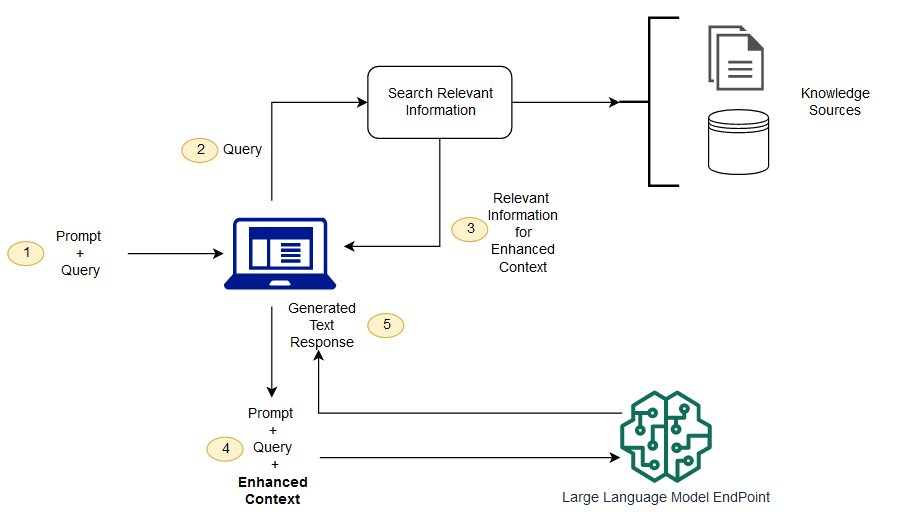
\includegraphics[width=0.85\textwidth]{figures/rag_workflow.jpg}
    \caption{Workflow général d'un système RAG \cite{aws_rag}}
    \label{fig:rag_workflow}
\end{figure}

\subsubsection{Agentic RAG}

L'\textit{agentic RAG} \cite{ibm_agentic_rag} désigne une évolution du RAG dans laquelle la récupération d'information n'est pas seulement déclenchée de manière automatique, mais pilotée par un ou plusieurs agents capables de décider quelles sources consulter, quels outils utiliser et comment intégrer les informations récupérées dans leur raisonnement. Cette approche rend le RAG plus flexible qu'un pipeline classique, car l'agent peut adapter la récupération au contexte de la requête.

\subsubsection{Utilisation dans le projet}

Dans la plateforme, l'Agentic RAG est utilisé pour les fonctionnalités nécessitant une forte contextualisation, notamment le coaching pédagogique, les recommandations, les défis personnalisés et l'exploitation de la mémoire des cours et des apprenants. Il permet aux agents de récupérer les informations pertinentes en fonction du contexte utilisateur et de l'objectif pédagogique.

Cette approche est plus adaptée qu'un RAG classique, car chaque agent (coaching, recommandation, défis) exploite un contexte différent. L'Agentic RAG permet ainsi d'adapter dynamiquement la récupération d'informations à chaque responsabilité, afin de produire des réponses plus cohérentes et personnalisées.

\subsection{Modèles d’Embeddings}

Les embeddings jouent un rôle central dans la recherche sémantique et le RAG.

Cette section en présente le principe et l’utilisation dans le projet.

\subsubsection{Définition des embeddings}

Les incorporations \cite{ibm_embedding}, ou embeddings, désignent des représentations vectorielles denses de données textuelles dans un espace mathématique de haute dimension. Elles permettent de représenter des objets, tels que du texte, des images ou de l'audio, sous forme de points dans un espace vectoriel continu dont la position porte une signification sémantique. Dans le cas du texte, la proximité géométrique entre deux vecteurs reflète ainsi une similarité de sens entre les éléments représentés.

\subsubsection{Embeddings et recherche sémantique}

Dans les systèmes basés sur les Transformers, les embeddings représentent des passages entiers et non seulement des mots isolés. Ils permettent ainsi la recherche sémantique, où le système compare le sens des requêtes et des contenus plutôt que des mots-clés exacts. Dans un système RAG, cette représentation sert à retrouver les fragments de connaissances les plus proches de la requête de l'utilisateur.

\subsubsection{Étude du choix du modèle d'embeddings}

Le choix du modèle d'embeddings influence la qualité de la recherche sémantique dans le système RAG. Une comparaison des principaux modèles est présentée dans le tableau~\ref{tab:comparaison_embeddings} selon plusieurs critères techniques et économiques.

\begin{table}[H]
\centering
\caption{Comparaison des modèles d'embeddings utilisables pour le système RAG}
\label{tab:comparaison_embeddings}
\renewcommand{\arraystretch}{1.25}
\resizebox{\textwidth}{!}{%
\begin{tabular}{|p{4.3cm}|p{3.2cm}|p{2.5cm}|p{7.0cm}|}
\hline
\textbf{Modèle} & \textbf{Fournisseur} & \textbf{Dimension} & \textbf{Coût et déploiement} \\
\hline
BAAI/bge-small-en-v1.5 \cite{baai_bge_small} & Local / SentenceTransformers & 384 & Gratuit à l'usage, exécution locale, modèle léger d'environ 130 Mo \\
\hline
text-embedding-3-small \cite{openai_embedding_models} & OpenAI & 1536 & Service cloud payant : 0,02 \$ / 1M tokens \cite{openai_embedding_pricing} \\
\hline
mistral-embed \cite{mistral_embed_models} & Mistral AI / LiteLLM & 1024 & Service cloud payant : 0,10 \$ / 1M tokens en entrée \cite{mistral_embed_model_card} \\
\hline
embed-english-v3.0 \cite{cohere_embed_models} & Cohere & 1024 & Service cloud avec clé API ; prix public par token non précisé pour ce modèle dans la page officielle \cite{cohere_pricing} \\
\hline
gemini-embedding-001 \cite{google_vertex_embeddings} & Google / Vertex AI & 3072 par défaut, dimension configurable & Service cloud : gratuit en free tier, puis 0,15 \$ / 1M tokens en entrée \cite{google_gemini_pricing} \\
\hline
\end{tabular}%
}
\end{table}

\subsubsection{Choix retenu}

À partir de cette comparaison, le modèle \textit{BAAI/bge-small-en-v1.5} a été retenu pour
la génération des embeddings dans le système RAG du projet. Ce choix s'explique par son
exécution locale, son coût nul à l'usage et sa légèreté, puisqu'il produit des vecteurs de
384 dimensions.

Ce modèle offre un compromis adapté entre qualité de recherche sémantique, consommation
mémoire et simplicité d'intégration. Les tests réalisés ont montré qu'il répond aux besoins de
récupération d'informations de la plateforme. Il est également cohérent avec le système de
mémoire utilisé dans le projet, qui supporte les embeddings locaux basés sur ce modèle
\cite{hindsight_models}.

\subsection{Les prompts système des agents IA}

Cette section présente les prompts système des agents IA ainsi que leur utilisation dans la plateforme.

\subsubsection{Définition}

Un prompt système \cite{kern_system_prompt} correspond à un ensemble de consignes placées
en amont de l'interaction avec le LLM. Il permet d'orienter le modèle avant même la demande
de l'utilisateur, en précisant le rôle attendu, les règles de comportement, le style de réponse,
les contraintes fonctionnelles et les limites à ne pas dépasser.

\subsubsection{Rôle dans les agents IA}

Dans une application basée sur des agents IA, le prompt système permet de spécialiser un
modèle généraliste afin qu'il adopte un comportement cohérent avec un contexte métier précis.
Chaque agent reçoit ainsi des consignes qui définissent son périmètre d'action, les informations
à prendre en compte et la forme attendue de sa réponse.

\subsubsection{Utilisation dans le projet}

Dans ce projet, les prompts système sont utilisés pour construire et spécialiser les agents de
coaching, de mémoire apprenant, de recommandation et de génération de défis. Ils permettent
également d'intégrer les éléments dynamiques nécessaires au raisonnement des agents, comme
l'historique de conversation, le profil de l'apprenant, le contexte du cours ou les mémoires
récupérées.

Ces prompts imposent aussi des formats de sortie structurés, notamment en JSON, afin que les
réponses générées soient directement exploitables par les services applicatifs de la plateforme.

La figure~\ref{fig:system_prompt_agent_recommandation} présente un exemple de prompt
système utilisé dans le projet pour encadrer l'analyse des difficultés de l'apprenant par
l'Agent de recommandation.

\begin{figure}[H]
\centering
\IfFileExists{figures/system_prompt_agent_defis.png}{%
    
\includegraphics[width=0.75\textwidth]{figures/system_prompt_agent_defis.png}
}{%
    \fbox{\parbox{0.85\textwidth}{\centering Capture du prompt système de l'Agent de recommandation à insérer ici.}}
}
\caption{Exemple de prompt système utilisé par l'Agent de recommandation}
\label{fig:system_prompt_agent_recommandation}
\end{figure}

\subsection{Les agent skills}

Cette section présente les agent skills et leur intégration dans la plateforme.

\subsubsection{Définition}

Les agent skills \cite{agent_skills_overview} désignent des blocs d'instructions spécialisés
qu'un agent peut utiliser pour traiter une tâche précise. Contrairement au prompt système,
qui définit le comportement général de l'agent, un skill apporte une logique plus ciblée :
il précise une méthode de raisonnement, des règles de décision ou une procédure adaptée à
un cas particulier.

\subsubsection{Besoin des skills dans le projet}

Dans le cadre de ce projet, l'utilisation des skills permet d'éviter de centraliser l'ensemble des règles de fonctionnement dans un seul prompt système. Cette approche rend les agents plus modulaires et facilite leur évolution.

Lorsqu'une tâche spécifique doit être exécutée, l'agent peut activer uniquement le skill correspondant, sans alourdir son contexte avec des instructions inutiles. Cela permet une meilleure séparation des responsabilités et une organisation plus claire du comportement des agents.

Ainsi, les skills contribuent à structurer les logiques de traitement de manière indépendante, tout en améliorant la maintenabilité et la flexibilité du système.

% ------------------------------------------------------------
\section{Système de mémoire persistante des agents IA}

La mémoire persistante permet aux agents IA de conserver et réutiliser des informations au-delà d'une seule session. Dans la plateforme, elle sert à exploiter le parcours de l'apprenant, ses interactions et les contenus déjà traités.

Cette section présente la solution retenue pour la gestion de cette mémoire, son fonctionnement et son intégration dans l'architecture de la plateforme.

\subsection{Présentation de Hindsight}

Hindsight \cite{hindsight_github} est un système de mémoire conçu pour les agents IA. Il fournit une couche dédiée à la mémorisation, à la récupération et à l'exploitation des informations retenues au fil des interactions, permettant ainsi de construire une mémoire durable et réutilisable.

Dans ce projet, Hindsight est retenu comme solution de mémoire persistante pour les agents IA, afin de conserver un contexte exploitable au fil des interactions et de renforcer la continuité des traitements.

\subsection{Architecture générale de Hindsight}

L'architecture de Hindsight repose sur deux niveaux principaux. Le premier correspond à la couche d'intégration, permettant aux agents de communiquer avec le système via une API, un SDK ou un client. Cette couche expose les opérations essentielles de gestion de mémoire telles que \textit{retain}, \textit{recall} et \textit{reflect}. Le second niveau est la couche de mémoire, organisée en \textit{memory banks} afin d'isoler les contextes selon l'utilisateur, le domaine ou le cours.

Au sein de chaque \textit{memory bank}, les informations sont structurées sous forme d'unités enrichies contenant des entités, des relations et des données temporelles. Ces éléments sont ensuite consolidés en différentes formes de connaissances, allant de faits simples à des représentations contextuelles plus globales (Figure~2.3).

\begin{figure}[H]
\centering
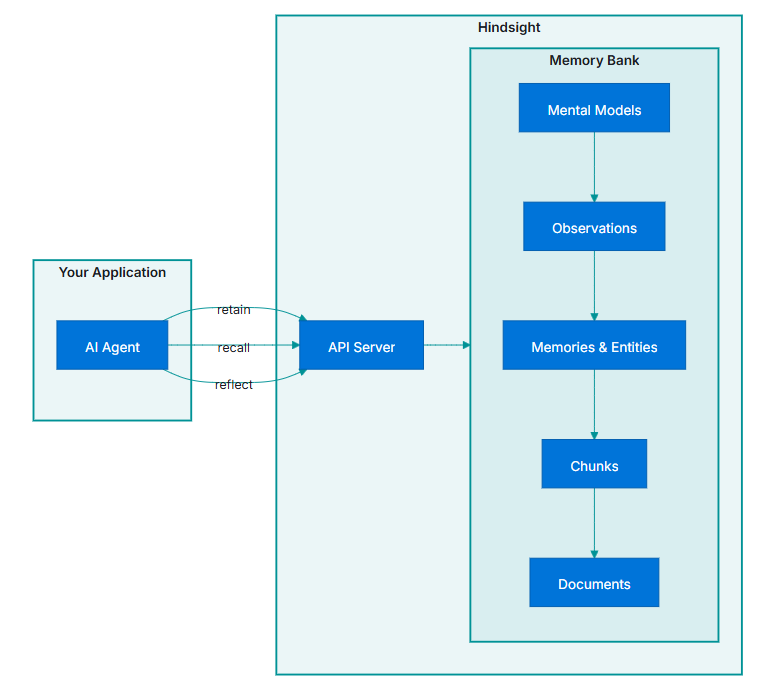
\includegraphics[width=0.75\textwidth]{figures/hindsight_architecture.png}
\caption{Architecture conceptuelle de Hindsight \cite{hindsight_homepage}}
\label{fig:hindsight_architecture}
\end{figure}

\subsection{Fonctionnalités fondamentales utilisées}

Dans le cadre du projet, Hindsight s'appuie sur trois opérations principales : \textit{retain}, \textit{recall} et \textit{reflect}, couvrant l'ensemble du cycle de gestion de la mémoire.

\textbf{Retain :} cette opération correspond à l'enregistrement des informations dans la mémoire. Comme illustré à la Figure~\ref{fig:hindsight_retain_architecture}, le système ne stocke pas le texte brut, mais exploite un LLM pour extraire les informations importantes (faits, entités, contexte temporel), puis les normalise afin d'éviter les doublons. Ces données sont transformées en \textit{memory units} enrichies par des métadonnées et des embeddings, puis organisées et classées en différentes catégories (\textit{world}, \textit{experience}, \textit{opinion}, \textit{observation}) avant stockage. Dans la plateforme, cette opération permet de conserver les interactions de l'apprenant, ses difficultés, ses erreurs récurrentes et ses préférences.

\begin{center}
    \IfFileExists{figures/hindsight_retain_architecture.png}{%
        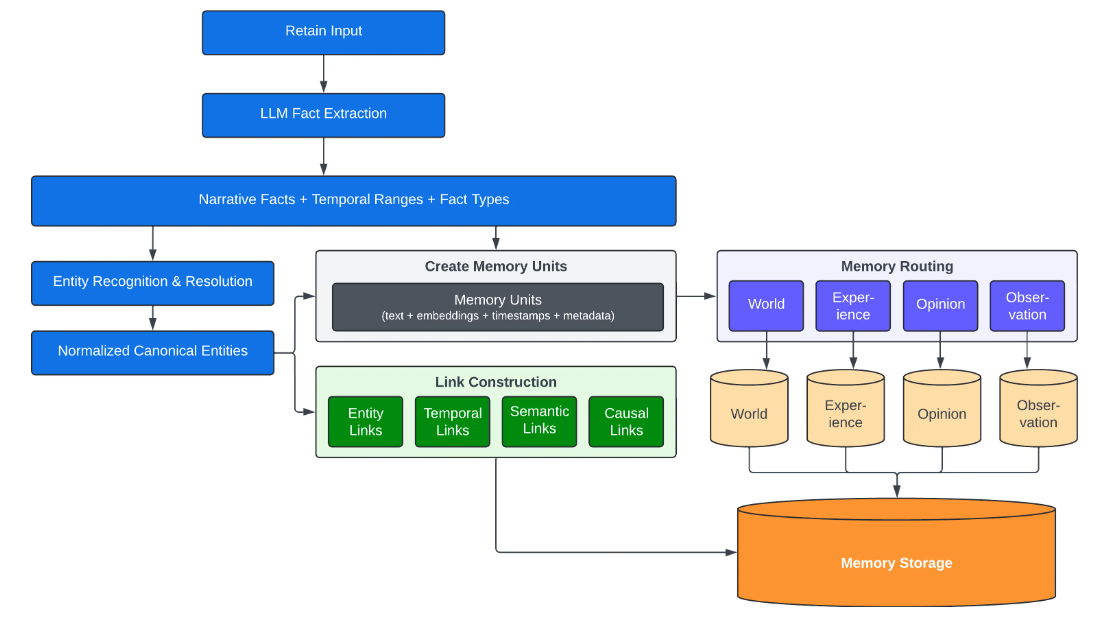
\includegraphics[width=0.98\textwidth]{figures/hindsight_retain_architecture.png}
    }{%
        \fbox{\parbox{0.85\textwidth}{\centering Schéma de fonctionnement de l'opération Retain à insérer ici.}}
    }
    \captionof{figure}{Fonctionnement de l'opération \textit{Retain} dans Hindsight \cite{hindsight_github}}
    \label{fig:hindsight_retain_architecture}
\end{center}

\textbf{Recall :} cette opération correspond à la récupération intelligente des mémoires déjà stockées. Comme l'illustre la figure \ref{fig:hindsight_recall_architecture}, Hindsight ne renvoie pas toute la mémoire à l'agent : il lance plusieurs recherches en parallèle, notamment la recherche sémantique par similarité vectorielle, la recherche par mots-clés, l'exploration des liens entre entités et l'exploitation des informations temporelles. Les résultats obtenus sont ensuite fusionnés, réordonnés et filtrés selon le budget de tokens disponible, afin de constituer un ensemble de souvenirs contextualisés à transmettre au LLM \cite{hindsight_recall}. Dans ce projet, \textit{recall} permet donc de retrouver les informations les plus utiles sur l'apprenant, son historique et le cours avant la génération d'une réponse.

\begin{center}
    \IfFileExists{figures/hindsight_recall_architecture.png}{%
        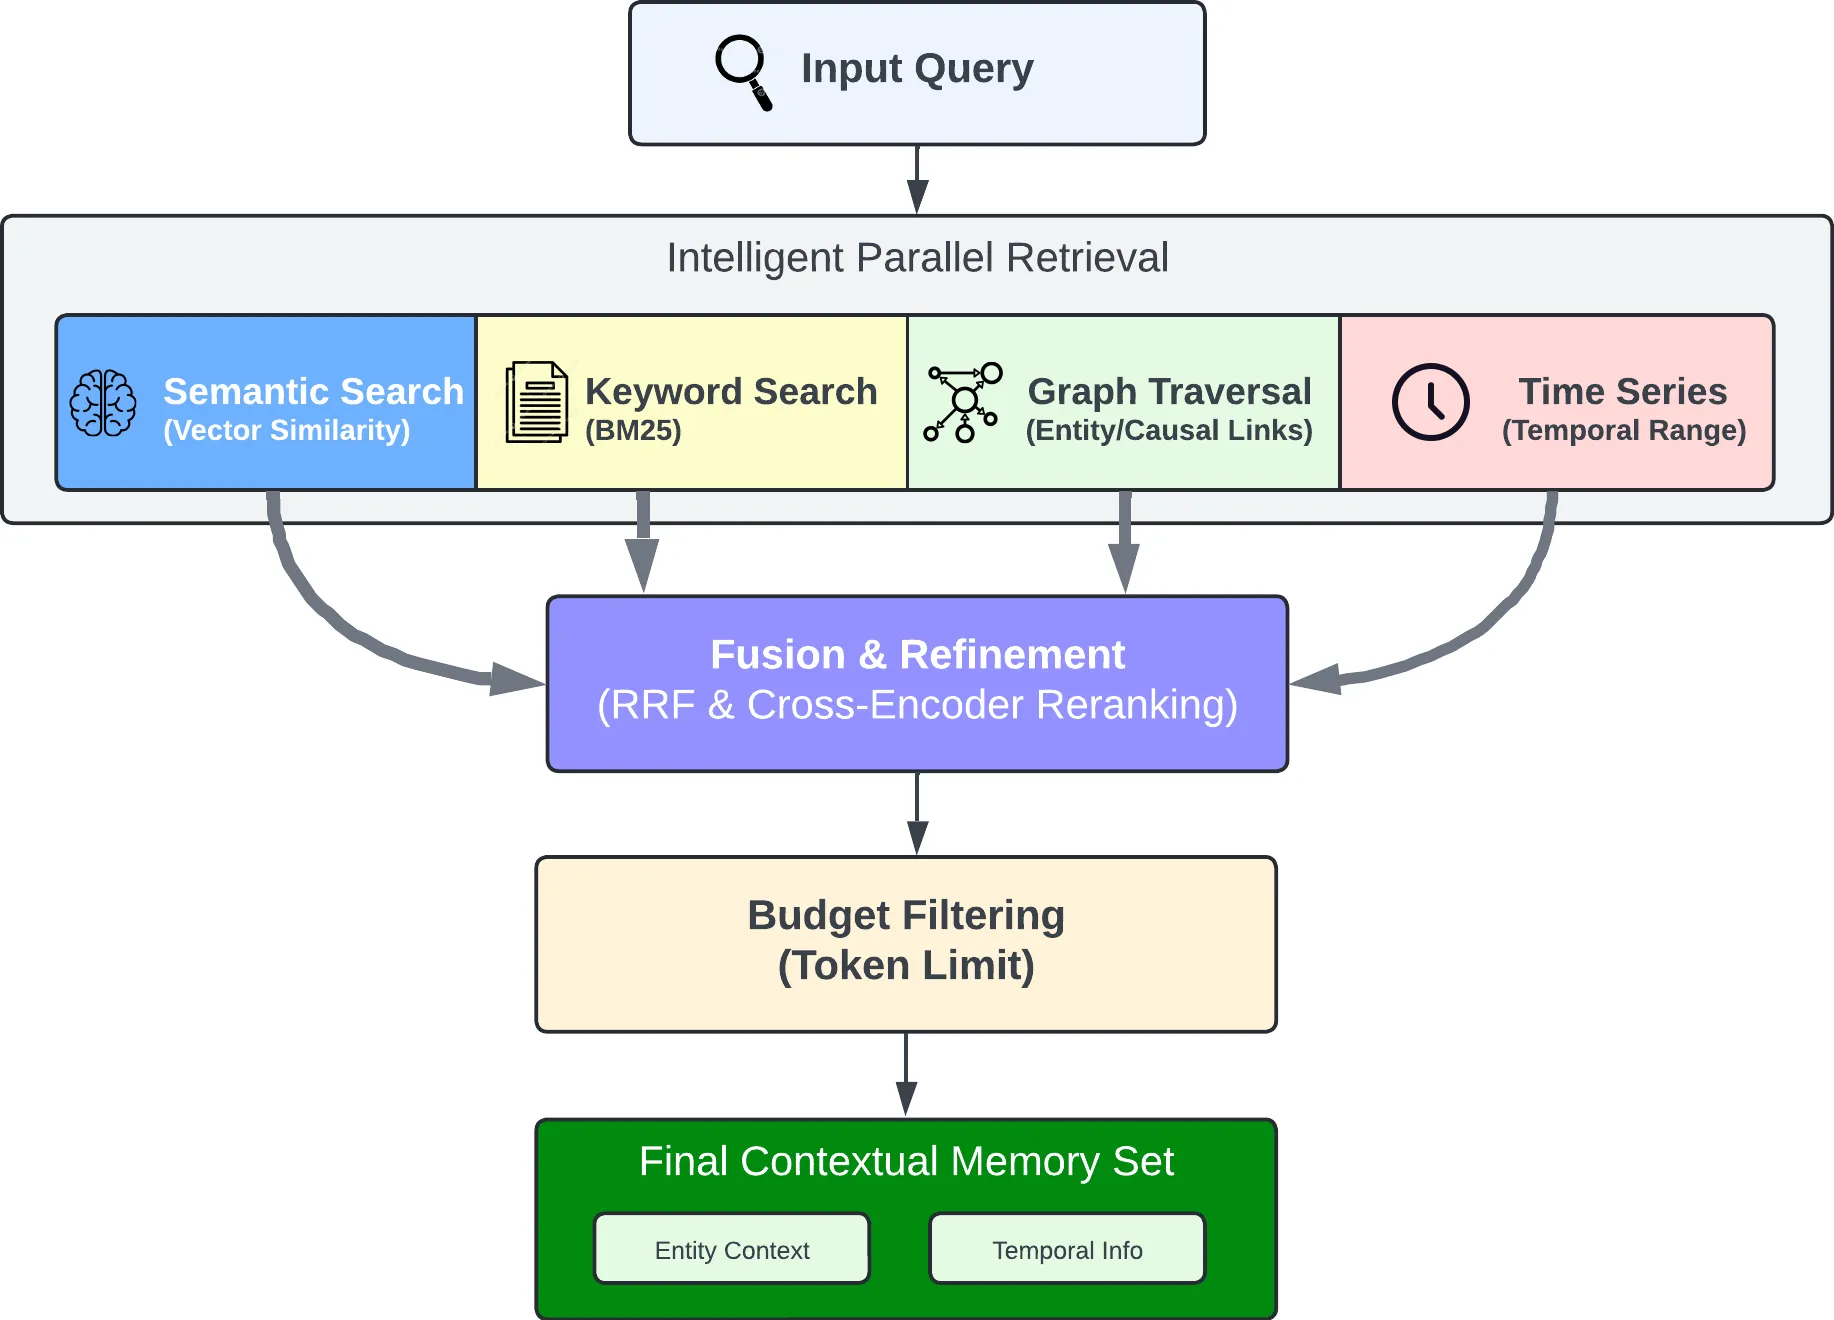
\includegraphics[width=0.9\textwidth]{figures/hindsight_recall_architecture.png}
    }{%
        \fbox{\parbox{0.85\textwidth}{\centering Schéma de fonctionnement de l'opération Recall à insérer ici.}}
    }
    \captionof{figure}{Fonctionnement de l'opération \textit{Recall} dans Hindsight \cite{hindsight_github}}
    \label{fig:hindsight_recall_architecture}
\end{center}

\noindent\textbf{Reflect :} cette opération correspond à la phase de réflexion et de mise à jour de la mémoire après une interaction. Comme l'illustre la figure \ref{fig:hindsight_reflect_architecture}, Hindsight récupère d'abord les mémoires pertinentes, construit un contexte, charge le profil de l'agent, puis utilise le LLM pour générer une réponse cohérente avec ce contexte. La réponse produite est ensuite analysée afin d'identifier de nouvelles observations ou de mettre à jour des opinions existantes, avec un niveau de confiance associé. Ces éléments sont réinjectés dans la mémoire persistante, ce qui permet à l'agent d'améliorer progressivement la cohérence de ses futures interactions \cite{hindsight_reflect}. Dans ce projet, \textit{reflect} est utile pour dégager des tendances sur le parcours d'un apprenant, consolider des observations pédagogiques et enrichir la mémoire des agents au fil des échanges.

\begin{center}
    \IfFileExists{figures/hindsight_reflect_architecture.png}{%
        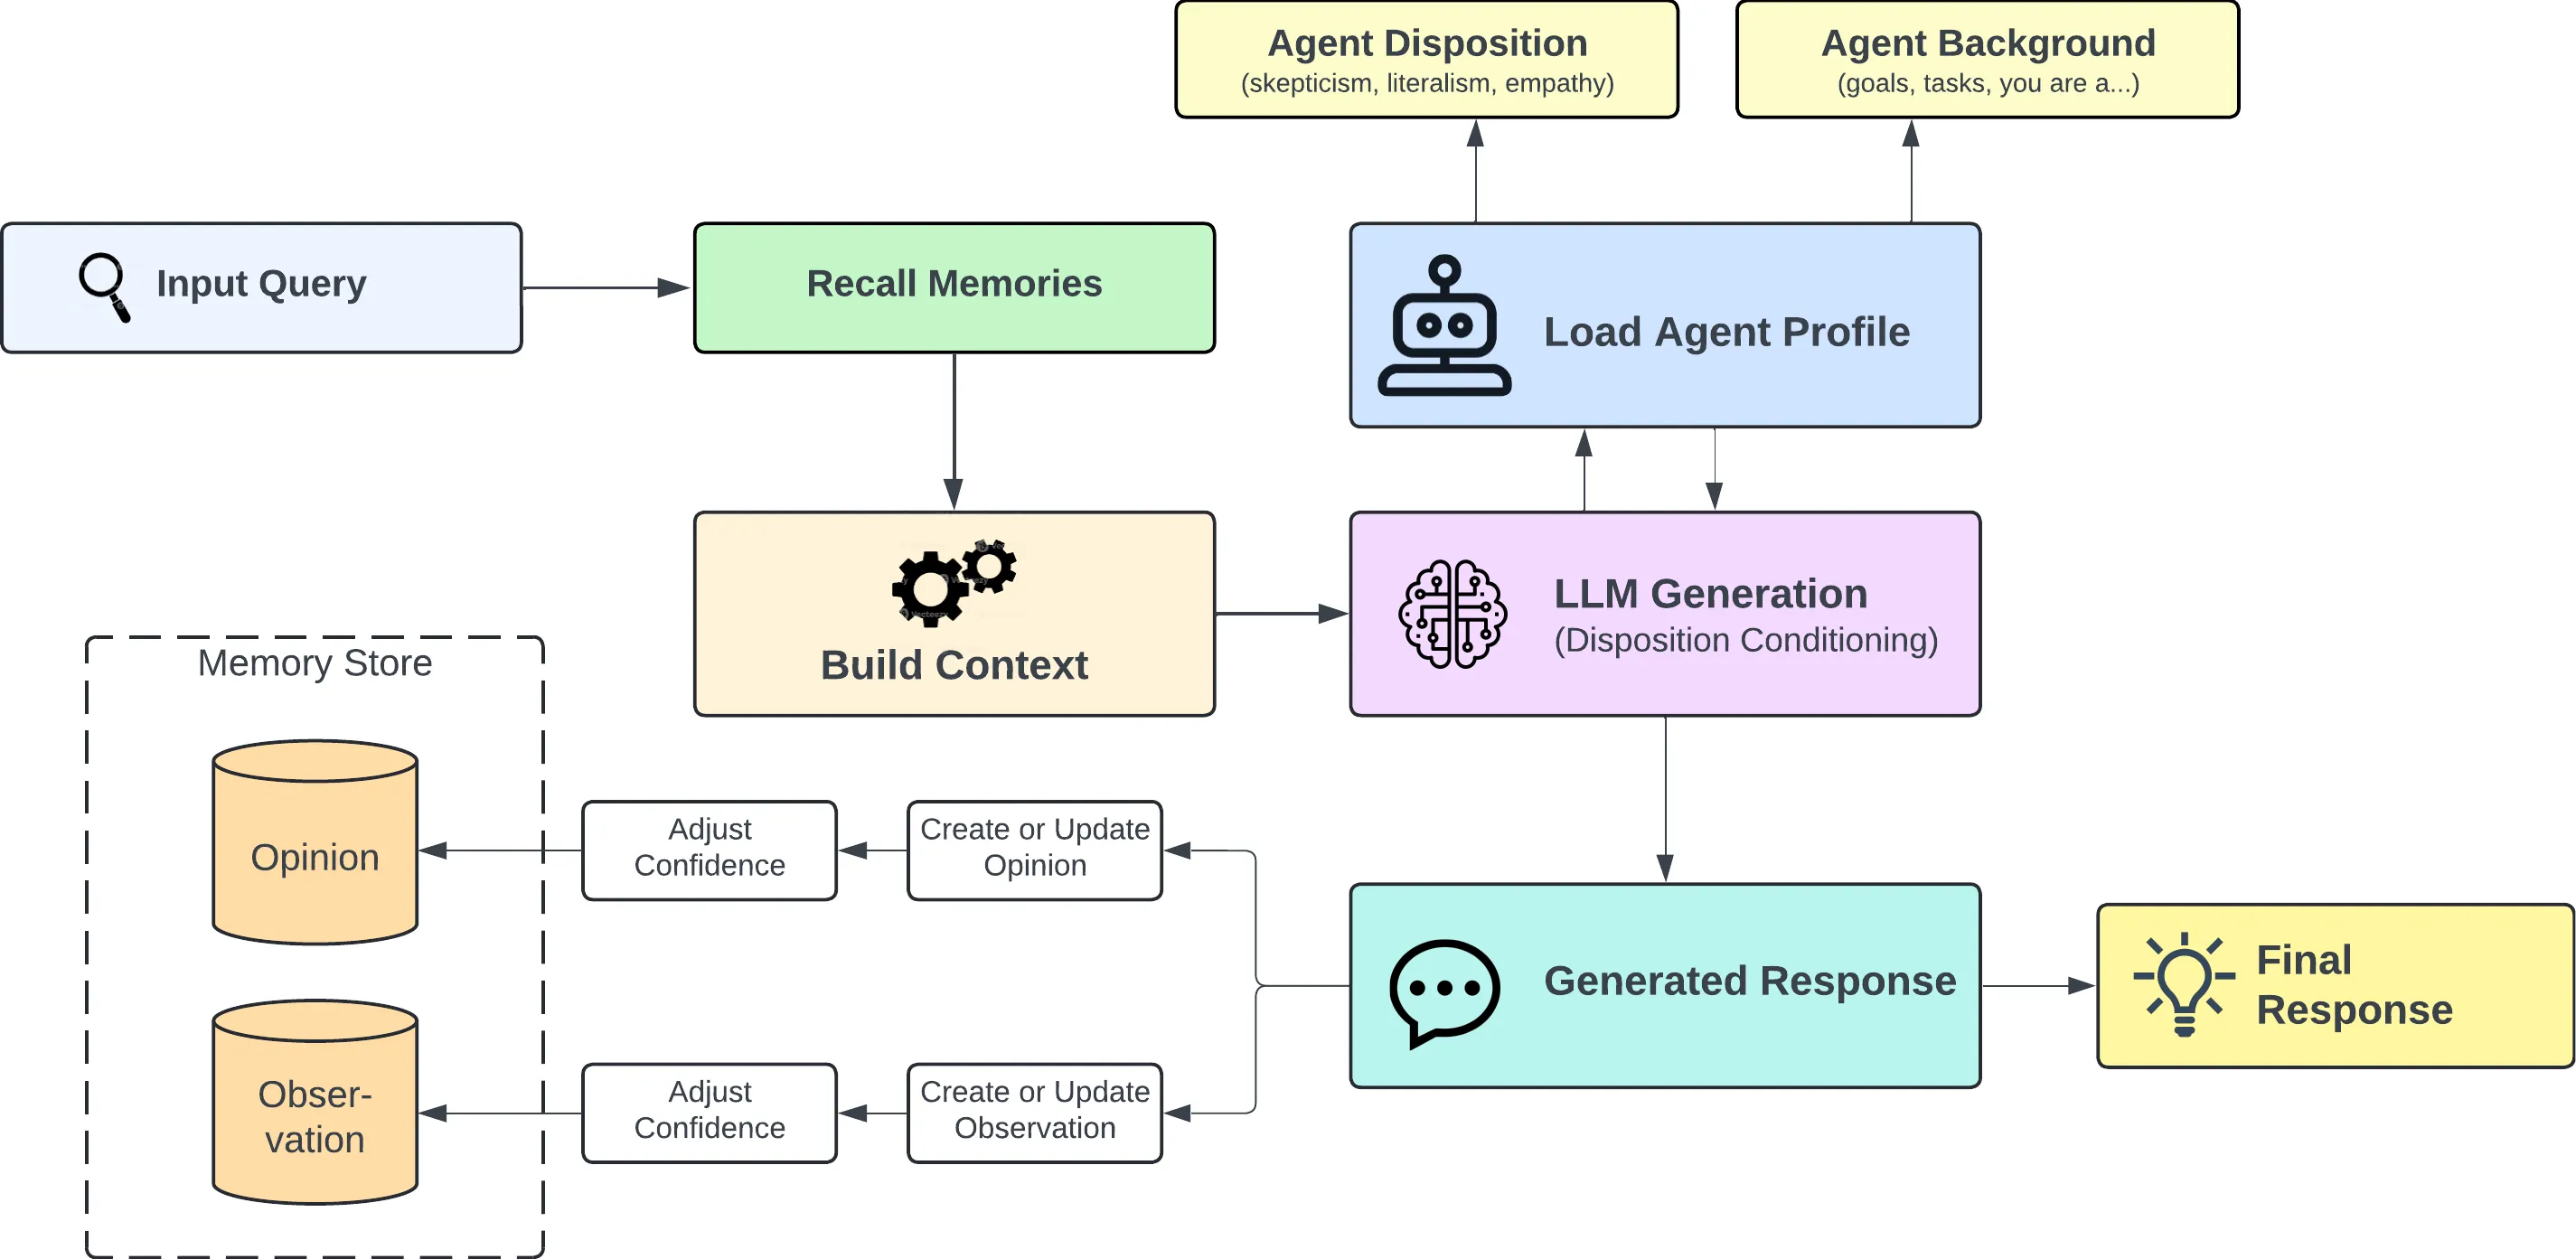
\includegraphics[width=0.9\textwidth]{figures/hindsight_reflect_architecture.png}
    }{%
        \fbox{\parbox{0.85\textwidth}{\centering Schéma de fonctionnement de l'opération Reflect à insérer ici.}}
    }
    \captionof{figure}{Fonctionnement de l'opération \textit{Reflect} dans Hindsight \cite{hindsight_github}}
    \label{fig:hindsight_reflect_architecture}
\end{center}

En résumé, l'organisation de la mémoire Hindsight repose sur un cycle continu qui permet
de conserver, d'exploiter et d'améliorer progressivement les informations utiles aux agents IA.
Cette approche donne à la plateforme une mémoire durable, capable de maintenir le contexte
au fil des interactions et de soutenir une personnalisation plus cohérente des réponses, des
recommandations et des activités proposées.



\subsection{Structure des mémoires persistantes dans Hindsight}

Dans ce projet, Hindsight organise les informations sous forme de \textit{memory banks} séparées, indexées à partir du \textit{tenantId}, du \textit{userId} et du \textit{courseId}. Cette organisation permet d'isoler les contextes (organisation, apprenant, cours) et d'offrir aux agents une mémoire structurée et ciblée. Le préfixe \texttt{tenant:\{tenantId\}} garantit également la cohérence avec l'architecture multi-tenant et évite tout mélange entre environnements.

On distingue principalement quatre types de banques mémoire :

\begin{itemize}
    \item \textbf{Banque de cours} \\
    \texttt{tenant:\{tenantId\}:course:\{courseId\}} \\
    Elle contient la mémoire pédagogique stable du cours (objectifs, leçons, quiz, supports, concepts). Elle est alimentée après la publication du cours et utilisée par les agents de coaching, recommandation et défis.

    \item \textbf{Banque apprenant-cours} \\
    \texttt{tenant:\{tenantId\}:user:\{userId\}:course:\{courseId\}} \\
    Elle regroupe l'historique de l'apprenant dans un cours (progression, résultats, erreurs, difficultés, interactions et retours).

    \item \textbf{Banque générale de l'apprenant} \\
    \texttt{tenant:\{tenantId\}:user:\{userId\}} \\
    Elle stocke les informations transversales comme les préférences pédagogiques, le profil et les connaissances générales.

    \item \textbf{Banque de profil de compétences} \\
    \texttt{tenant:\{tenantId\}:user:\{userId\}:skill-profile} \\
    Elle contient une synthèse des compétences et des écarts, utilisée principalement par l'Agent de recommandation pour éviter les recalculs.
\end{itemize}

Ainsi, cette structuration sépare clairement les connaissances liées au cours, au parcours utilisateur et aux compétences. Elle améliore la lisibilité de la mémoire, limite les ambiguïtés et permet aux agents de sélectionner directement le contexte pertinent selon leur objectif.


\section{Conclusion}

Ce chapitre a permis de poser les bases théoriques nécessaires à la compréhension de la solution proposée. Ces fondements constituent le socle sur lequel repose l'ensemble des mécanismes d'intelligence et d'interaction de la plateforme.

Ils offrent ainsi une vision claire des principes qui guident la conception et la mise en œuvre du système dans la suite du projet.



% =========================
% BIBLIOGRAPHIE
% =========================

\clearpage
\chapter*{Bibliographie}
\markboth{Bibliographie}{Bibliographie}
\addcontentsline{toc}{chapter}{Bibliographie}
\nocite{*}
\printbibliography[heading=none, notkeyword=web]

% =========================
% WEBOGRAPHIE
% =========================

\clearpage
\chapter*{Webographie}
\markboth{Webographie}{Webographie}
\addcontentsline{toc}{chapter}{Webographie}
\printbibliography[heading=none, keyword=web]

\appendix

\end{document}
